\documentclass[twocolumn,a4j,10pt]{jsarticle}
\usepackage[top=25truemm,bottom=25truemm,left=20truemm,right=20truemm]{geometry}

\usepackage[dvipdfmx]{graphicx}
\usepackage{amsmath}
\usepackage{url}
\usepackage[sectionbib]{chapterbib}
\usepackage{setspace}
\usepackage{theorem} 
\usepackage{fancyhdr}
\usepackage{multirow}
\usepackage{arydshln}
\usepackage{algorithm}
\usepackage{algorithmic}
\usepackage[thinlines]{easytable}
\usepackage[skip=0pt]{caption}
\mathchardef\mhyphen="2D

\newcommand{\eqnsp}{1em}
\newcommand{\vvspace}{\vspace*{1em}}
\newcommand{\mvspace}{\vspace*{-0.1em}}
\renewcommand{\bibname}{参考文献}
\usepackage[dvipdfmx]{hyperref}
\hypersetup{colorlinks=false}
\hypersetup{pdfborder={0 0 0}}

\usepackage{hypcap}
\usepackage{cite}
\usepackage{cleveref}



\begin{document}

\twocolumn[
2016.03 技術経営戦略学専攻 修士論文概要

\begin{center}
{\Large \bf 深層学習を用いたMOOCsの学習者の知識構造の分析}
\end{center}

\begin{flushright}
37-146856 那須野薫\\
指導教員 松尾豊特任准教授
\end{flushright}


]


\normalsize

\renewcommand{\baselinestretch}{1} 
\setstretch{1}
 
\section{研究背景および目的}
%心理学における知識の登場
伝統的に,知識は学習や指導の設計において重要な役割を担っており,心理学では知識について多角的に議論が行われていた.
知識の属性や性質から知識を比較する研究や,
学習者の知識の獲得や活用の仕組みを説明する研究,
また,それらを基に効率的な知識獲得の方法を開発する研究,
など幅広い.


%★ 宣言的知識と手続き的知識の登場.
知識の属性や性質という点では,
一般知識と領域知識,
宣言的知識と手続き的知識,
具体的知識と抽象的知識,
暗黙知,メタ知識など,さまざまな属性や性質,あるいはその対比を切り口に議論が行われてきたが,
このなかでも,宣言的知識と手続き的知識を対比し知識を議論する研究は多い.
宣言的知識は内容や概念を表現する知識であり,
{\it knowing that}という言葉でも表現され,対象(A)がどう(B)であるかに関する知識である.
例えば,「東京は日本の首都である」という知識が該当し,この場合,Aが東京であり,Bが日本の首都である.
一方で,
手続き的知識は,手続きを表現する知識であり,
{\it knowing how}という言葉でも表現され,タスクをどう達成するかに関する知識である.
特に,数学やプログラミングを対象に議論されることが多い.
例えば,「1次方程式$ax + b = 0$を解く」ための知識が該当し,この場合,
$b$を移行し$a$で両辺を割るという手続きにより問題を解くことができる.
知識を宣言的知識と手続き的知識に分けて議論することで,
人間の知識の獲得や活用を
内容と内容を基にした手続きでよく記述できる.


%★ 宣言的知識と手続き的知識の知識の獲得の違い.
特に,
学習者の知識獲得の点でも,
宣言的知識と手続き的知識を対比的に扱い説明する研究は多い.
宣言的知識は,
学習者が保有する知識に結合する形で獲得されるため,
獲得対象の知識に既に獲得しているものが含まれている方が獲得されやすい
といわれている.
例えば,「東京は日本の首都である」という知識であれば,
東京,首都,日本のうち,より多くについて既知であるほど獲得しやすく,
逆に,「地球は丸い」という知識が獲得していたとしても必ずしも獲得しやすいわけではない,
ということである.
一方で,手続き的知識は,
タスクが複数の細かいサブタスクに分解されるため,
学習者が分解後の全てのサブタスクを達成するための知識を保有している場合に獲得される
といわれている.
「1次方程式$ax + b = 0$を解く」ための知識は,
「項を移行する」ための知識と「両辺を定数で割る」ための知識に分解され,
さらに,「ある定数を引く」ための知識や「ある定数で割る」ための知識に分解され,
というように階層的に分解された知識を全て保有している場合に,
はじめて「1次方程式$ax + b = 0$を解く」ための知識を獲得しているといえる,ということである.
宣言的知識と手続き的知識はその獲得のされやすさが学習者が既に獲得している知識に依るところは共通するが,
宣言的知識は関連の強い知識間で局所的にその獲得に影響を与え合い,
一方で,手続き的知識は分解された知識がその掛け合わせで構成される知識の獲得に影響を与えるため,
知識獲得における知識構造は,手続き的知識のものは宣言的知識のものと比べると,階層的になると考えられていた.


心理学の領域で,この考えを支持する研究報告は少なくない.
領域知識をよく分析し階層的に知識間関係を構築し,
階層構造上より水準の高い知識に着手する前に,予め獲得するべき知識が確実に獲得されるように学習体験を構造化することで,
習熟学習を効率化できるという仮説に基づいて,
数学やプログラミングの習熟の効率化を狙った研究が報告された.
こうした研究は,
当初の期待よりは効果が低かったものの,
よく分析し階層的に構造化した知識間関係に基づいて学習を設計することで学習を効率化できることを実験で示し,知識獲得における対象科目の知識構造が階層的であることを示唆するというものであった.


しかし,実験より示唆する研究報告はあるものの,
宣言的知識と手続き的知識の対比において,知識獲得における知識構造を定量的に比較し分析した研究はまだない.
これは,こうした心理学の研究が行われていたのが20年以上も前で,
当時は,定量評価を実施できる学習者の知識獲得に関するデータの収集が困難であり,
知識獲得に関するデータから知識獲得における知識構造を抽出することも難しく,
また,抽出した知識構造を分析する方法もなかったからだと推察される.



さて,こうした知識間関係のように対象間の関係を明らかにしようとする分析として,ネットワーク分析というものがある.
ネットワーク分析はウェブやそれソーシャルメディアの普及に伴い注目が高まり,ウェブページ間の関係や人と人の関係を分析するためにしばしば用いられている.
ネットワーク分析は対象をノード,対象間の関係をエッジとするグラフを構築し,その構造から関係を評価しようというものである.
ネットワークの構造を捉えるための指標や手法が開発されており,
例えば,ネットワークのモジュール性を評価するモジュラリティ\cite{newman2006modularity}という指標や
階層性を評価するフロー階層\cite{luo2011detecting}やGRC\cite{mones2012hierarchy}という指標
等,多くの指標がある.



また,学習や教育に関する領域では,近年,Massive Open Online Courses(以下,MOOCs)が注目を集めている.
MOOCsは,
従来の教室で時間割通りに一斉授業形式で提供される学習機会とは異なり,
数多くの多様な講座のオンライン上での提供を通じて,
いつでもどこでも自分のペースでさまざまな講座から自分の学習したいものを選択し学習できるというこれまでにない学習機会を提供しており,
多くの学習者が利用している.


MOOCsは単にこれまでにない学習機会を提供しているというだけでなく,
これまで難しかった大規模な学習効果分析の可能性も高めている.
学習者はオンライン上で提供された講義動画や演習問題を通して学習するが,
オンライン上で実施されているため学習行動ログをデータとして蓄積でき,さらに,そのデータを分析に活用できる.
また,多くの多様な学習者が利用するため,多様な学習者の大規模な学習行動ログから多様な講座の学習効果の分析が可能となりつつある.
特に,演習問題の回答ログはその演習問題により評価される知識を学習者が獲得しているか否かを表現しているため,知識獲得の分析に利用できる.


%登場
また,ここ数年,多くの研究領域で深層学習が注目されている.
深層学習は多層のニューラルネットワークによる機械学習のことで,
従来の機械学習では難しかった対象データの表現抽出を最適化の過程で行うことができる.
深層学習の活用により画像認識,機械翻訳,質問応答文生成,音声認識等さまざまな研究領域で飛躍的な進展が報告がされている.


特に,学習者の知識獲得を予測する研究も,深層学習により大きく進展している.
2015年に,数学における知識獲得の予測に深層学習を活用し,
高い精度で知識獲得を予測できること,
予測モデルを分析することで知識間関係をネットワークとして抽出できることが報告された\cite{piech2015deep}.
学習者が獲得している知識から,ある知識の獲得されやすさをそのまま予測しており,
得られた知識間関係から抽出したネットワークは知識獲得における知識構造を表現しているといえる.


これまで,心理学で議論されていたものの定量的な分析が困難だった宣言的知識と手続き的知識の獲得における知識構造の違いは,
MOOCsの登場によりさまざまな科目について問題回答ログがデータとして蓄積されるようになり,
その蓄積された学習者の知識獲得の軌跡から深層学習により知識間関係を抽出できるようになり,
さらに,ネットワーク分析の発展により抽出した知識構造を分析できるようになった今,
定量的に分析できる可能性が高まっている.



本論文の目的は,
心理学で議論されていた宣言的知識と手続き的知識の獲得における知識構造の違いを定量的に分析することとで下記の2つを検証することである.
\begin{itemize}
\item 知識獲得における宣言的知識の知識構造は手続き的知識の知識構造と比べてよりモジュール性が高い.
\item 逆に,知識獲得における手続き的知識の知識構造は宣言的知識の知識構造と比べてより階層性が高い.
\end{itemize}

従来心理学で議論され,実際の教育や学習にも活用されているものの,
定量的に検証されていないこれら知識構造について明らかにすることは,学術的な意義が大きいと考える.

\section{先行研究}
\subsection{Massive Open Online Courses}
% - MOOCsについて,5W1Hを明らかにする
Massive Open Online Courses(以下,MOOCs)は
オンライン上で誰もが受講できる大規模な講座群のことで,
参加人数が非常に大規模であるという点や,高等教育水準の内容の講座だけでなく初等中等教育水準の内容の講座も含まれるという点でオープンコースウェアやこれまでのオンライン講座とは異なる.
従来の教室で時間割通りに一斉授業形式で提供される学習機会とは異なり,
いつでもどこでも自分のペースでさまざまな講座から自分の学習したいものを選択し学習できるというこれまでにない学習機会を提供している.

さらに,MOOCsには
これまで難しかった大規模な学習効果分析の可能性を高めるという側面もある.
特に,演習問題の回答ログはその演習問題により評価される知識を学習者が獲得しているか否かを表現しているため,知識獲得の分析に利用できる.

\subsection{深層学習}
% - RNNの構造の概略

知識獲得の予測に深層学習を用いた手法\cite{piech2015deep}に用いられていたニューラルネットワークであるRecurrent Neural Networks(以下,RNN)について説明する.
%近年,RNNはデータの大規模化や計算機性能の向上により機械翻訳,音声認識,医療診断等幅広い領域の系列データに対して適用されるようになった.
伝統的なRNNの構造は,
入力層,隠れ層,出力層の3層から構成されている.
系列方向を時刻とすれば,
時刻$t$の隠れ層${\bf h}_t$の計算に時刻$t-1$の隠れ層の情報を入力する${\bf h}_t = f({\bf x}_t, {\bf h}_{t-1})$の式ように,一つ前の情報を繰り返し入力するという構造である.

RNNには異なる活性化関数を利用するという形でいくつかの種類がある.
特に,本研究で用いるGated Recurrent Neural Networks(以下,GRNN)\cite{cho2014learning}について説明する.
GRNNはGated Recurrent Unit\cite{cho2014learning}というゲート付き活性化関数を用いるRNNのことで,
GRUは,長期的な表現と短期的な表現を捉えるために開発された.
GRNNは下記の式により定義される.
${\bf x}_t$は入力ベクトル,
${\bf W}_{xr}, {\bf W}_{hr}, {\bf W}_{xz}, {\bf W}_{hz}, {\bf W}_{xh}, {\bf W}_{hh}$は重み行列, 
${\bf b}_r, {\bf b}_z, {\bf b}_h$はバイアス項である.
\begin{eqnarray}
\label{eq:grurnn1}
{\bf r}_t &=& \sigma({\bf W}_{xr}{\bf x}_t + {\bf W}_{hr}{\bf h}_{t-1} + {\bf b}_r)\\
\label{eq:grurnn2}
{\bf z}_t &=& \sigma({\bf W}_{xz}{\bf x}_t + {\bf W}_{hz}{\bf h}_{t-1} + {\bf b}_z)\\
\label{eq:grurnn3}
\tilde{{\bf h}}_t &=& \tanh({\bf W}_{xh}{\bf x}_t + {\bf W}_{hh}({\bf r}_t \odot {\bf h}_{t-1} + {\bf b}_h))\\
\label{eq:grurnn4}
{\bf h}_t &=& {\bf z}_t \odot {\bf h}_{t-1} + (1 - {\bf z}_t) \odot \tilde{{\bf h}}_t\\
\label{eq:grurnn5}
{\bf y}_t &=& \sigma( {\bf W}_{hy} {\bf h}_t + {\bf b}_y)
\end{eqnarray}




\subsection{知識獲得の予測}
知識獲得の予測は,学習者が対象の知識を獲得しているか否かを予測するというものである.
通常,知識を獲得しているか否かは問題回答の正誤を基に評価されるため,
知識獲得の予測のタスクは過去の学習者の問題回答履歴から次に解く問題の正誤を予測するというものである.
最初の定式化の事例は,1994年に報告されたKnowledge Tracing\cite{corbett1994knowledge}である.
Knowledge Tracingは,
学習者の時刻$t$において観測された問題回答結果を$q_{t}$とすれば,
$q_1, q_2, \dots, q_t$から時刻$t+1$において観測される問題回答結果$q_{t+1}$を予測するタスクである.
特に,回答の正誤確率を算出する場合は,
$q_1, q_2, \dots, q_t$が観測された場合の時刻$t+1$に着手する問題において当該学習者の回答が正解となる事後確率
$p(q_{t+1} = correct|q_1, q_2, \dots, q_t)$を求めるタスクである.


Bayesian Knowledge Tracing\cite{corbett1994knowledge}(以下,BKT)はベイズの定理の事前確率と事後確率の関係に基づいて正解確率をモデル化する手法である.
スキルごとに4つの確率変数が定義されており,これらを組み合わせてスキルの習熟をモデル化している.
習熟,つまり時系列性を捉える手法であり,知識間関係は考慮しない.
 
Deep Knowledge Tracing\cite{piech2015deep}(以下,DKT)はRNNを利用しKnowledge Tracingを行う手法である.
2015年6月に発表され,
高い性能で知識獲得を予測できること,
予測モデルを分析することで知識間関係をネットワークとして抽出できることが報告された.

DKTの構造は伝統的なRNNの構造に基づいている.
\begin{eqnarray}
\label{eq:rnn1}
{\bf h}_t &=& f({\bf x}_t, {\bf h}_{t-1})\\
\label{eq:rnn2}
{\bf y}_t &=& g({\bf h}_t)
\end{eqnarray}
モデルは関数$f$と$g$によって定義されており,
本研究では,関数$f, g$にGRNNの式\ref{eq:grurnn1}--\ref{eq:grurnn5}を利用する. 

\begin{table}[tb]
\caption{Deep Knowledge Tracingにおける回答ログデータと対応する入力ベクトルの例}
\label{tab:samplelog}
\begin{center}
\centerline{
{\scriptsize
\begin{tabular}{ccc|cc}\hline\hline
	\multicolumn{3}{c|}{回答ログ}	&	\multicolumn{2}{c}{入力ベクトル}	\\
		ログの順番	&	問題番号	&	正誤	&	変数名			&	値											\\\hline
		1			&	1			&	0		&	${\bf x}_1$ 			& $[0 0 0 0 \hspace{1mm} 1 0 0 0 ]$	\\
		2			&	1			&	1		&	${\bf x}_2$ 			& $[1 0 0 0 \hspace{1mm} 0 0 0 0 ]$	\\
		3			&	2			&	1		&	${\bf x}_3$ 			& $[0 1 0 0 \hspace{1mm} 0 0 0 0 ]$	\\
		4			&	3			&	0		&	${\bf x}_4$ 			& $[0 0 0 0 \hspace{1mm} 0 0 1 0 ]$	\\
		5			&	3			&	1		&	${\bf x}_5$ 			& $[0 0 1 0 \hspace{1mm} 0 0 0 0 ]$	\\
		6			&	4			&	1		&	${\bf x}_6$ 			& $[0 0 0 1 \hspace{1mm} 0 0 0 0 ]$	\\
\hline\hline
\end{tabular}
}
}
\end{center}
\vspace*{-5mm}
\end{table}
DKTの入力は, 
学習者の学習行動の観測結果をone-hotベクトルに符号化したもの${\bf x}_t$をを用いる.
観測結果は演習問題と正誤の組み合わせで表現できるため,演習問題の数を$M$とすれば,${\bf x}_t$の長さは$2M$となる.
例えば,回答ログと対応する入力ベクトルは表\ref{tab:samplelog}のにようになる.
出力${\bf y}_t$は問題数と同じ長さのベクトルで,
それぞれの要素が当該学習者がそれぞれの問題に正しく回答する確率の予測値となっている.
モデルは誤差関数を負の対数尤度とし,確率的勾配降下法で学習させる.


DKTによる知識間関係抽出法について述べる.
%次に,DKTのモデルを利用した知識間関係(あるいは,問題間関係)抽出法について述べる.
問題$i$と$j$のすべての有向ペアのうち,
問題$i$が出現した後に残りの問題系列の中で問題$j$が出現する系列数が問題$i$が出現する問題系列数全体の$1\%$以上であるものに対して,
影響度
$J_{ij} = \frac{y(j|i)}{\sum_k y(j|k)}$
を割り当てる.
ここでは,$y(j|i)$は,ある学習者が最初に問題$i$に正答した場合に,RNNによって割り当てられる次の時刻に問題$j$に正答する確率である.
ネットワークは,影響度が$0.1$以上であればエッジを引くというようにして構築された.
得られたネットワークは,
単に学習者の問題$(i, j)$間の遷移率から構築したネットワークや
問題$i$の正解が観測された後に問題$j$の正解が観測される条件付き確率から構築したネットワークより
よく知識間関係を捉えていることが指摘されている.
こうして得られた行列$J$は,
問題$i$で評価される知識が既に獲得されている場合に,
問題$j$で評価される知識の獲得されやすさを表現しており,
$J$は知識間関係行列であるといえ,
この知識間関係行列から構築したネットワークは
知識獲得における知識構造を表現していると考えられる.





\subsection{ネットワーク分析}
ネットワーク構造を評価する指標について述べる.
モジュラリティ\cite{newman2006modularity}はネットワークのクラスタへの分割におけるモジュール性を評価するという指標で式\ref{eq:modularity}で与えられる.
ここでは,
$e_{ii}$はクラスタの隣接行列の$(i, i)$成分を,
$a_i$は隣接行列の$i$行の和を
示す.
この指標はクラスタ内のエッジ割合とクラスタ間のエッジ割合の差を表現した指標だといえる.
\begin{eqnarray}
	\label{eq:modularity}
	Modularity &=& \sum_i(e_{ii} −a^2_i)
\end{eqnarray}

フロー階層\cite{luo2011detecting}は式\ref{eq:flowhierarchy}で与えられる.
ここでは,
$L$はネットワークに含まれるエッジの数を,
$e_{i}$はエッジ$i$が環状構造に含まれていたら$e_{i}=0$でそれ以外は$e_{i}=1$となるような指標を示す.
この指標は
階層性を,環状構造がない,という側面から捉えようとした指標だといえる.
\begin{eqnarray}
	\label{eq:flowhierarchy}
	FlowHierarchy &=& \frac{\sum^L_{i=1}e_{i}}{L} 
\end{eqnarray}


GRC\cite{mones2012hierarchy}はGlobal Reaching Centralityのことで,式\ref{eq:grc}で与えられる.
ここでは,
$C_R(i)$がLocal Reaching Centralityという指標を,
$V$はネットワークに含まれるノードの集合を,
$C_R^{max}$は$V$に含まれる全ノード$i$について$C_R(i)$の最大値を,
$N$は$V$の大きさであるノード数を示す.
$C_R(i)$はノード$i$から出力されるエッジを辿って,ノード$i$から到達できるノードの割合を指す.
この指標は階層性を
一部のノードが他のノードより到達できるノードが多い構造にある,という側面から捉えようとして指標だと言える.
\begin{eqnarray}
	\label{eq:grc}
	GRC &=& \frac{\sum_{i\in V}[C^{max}_R - C_R(i)]}{N-1}
\end{eqnarray}





\section{分析手法}

\begin{figure}[tb]
\begin{center}
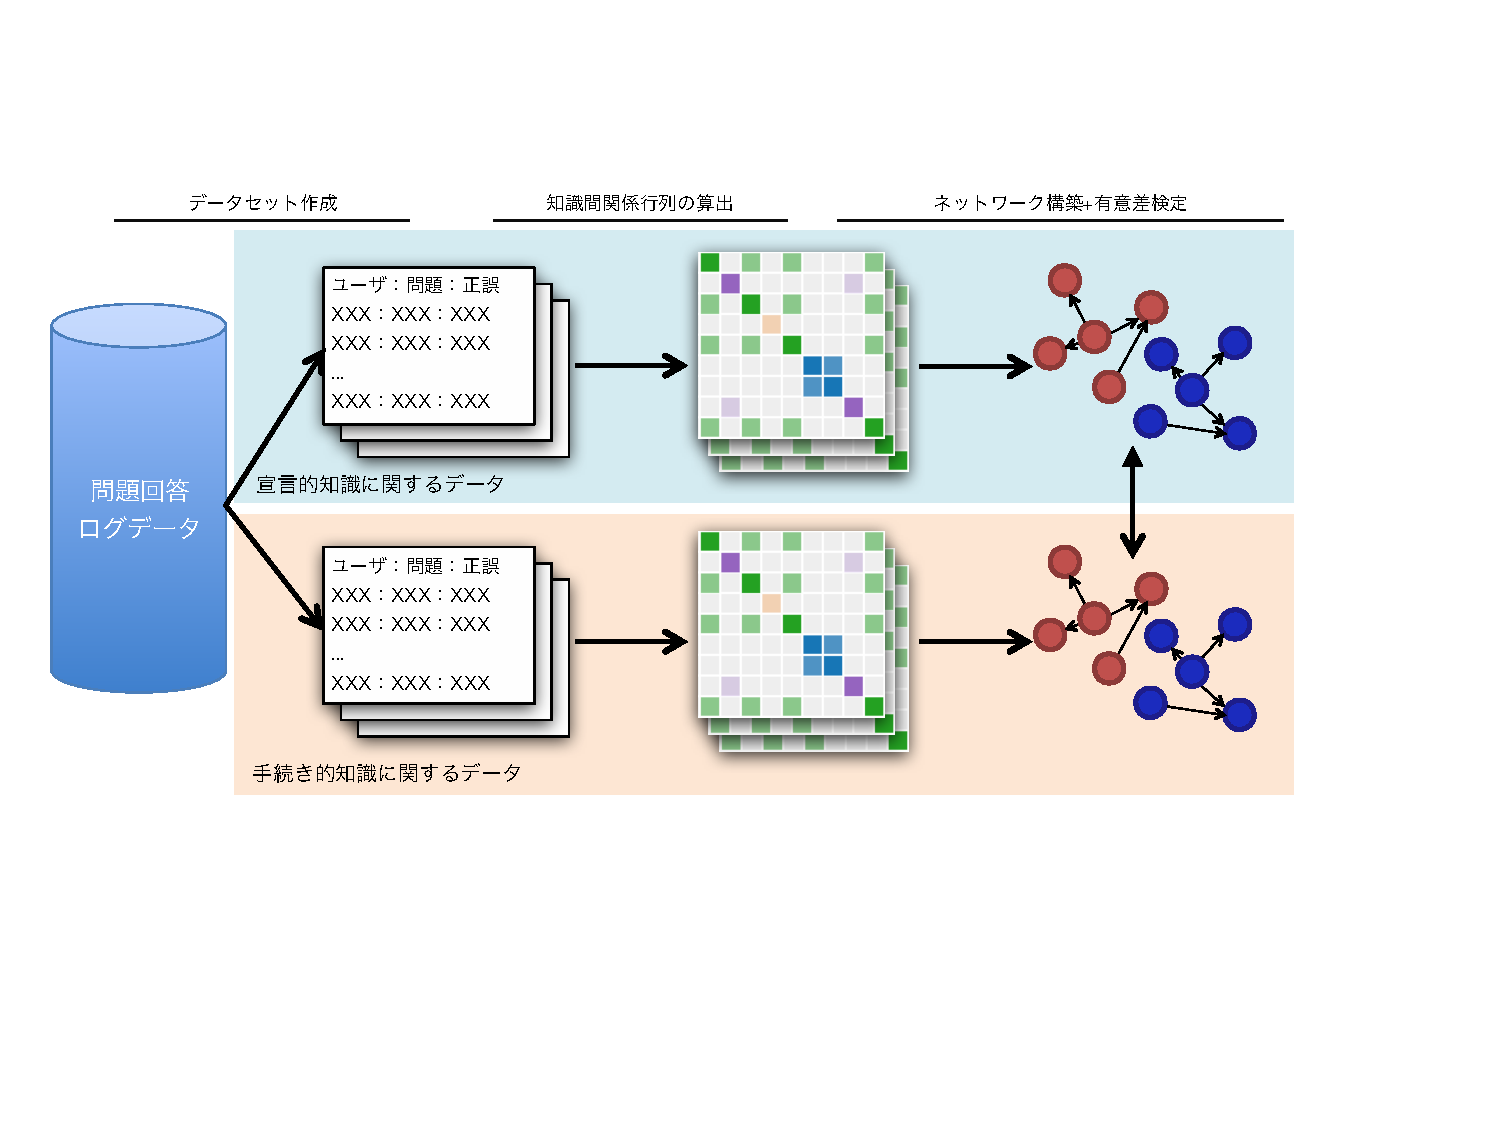
\includegraphics[width=240pt]{./img/method2.pdf}
\end{center}
\caption{分析手法全体の流れ}
\label{fig:method}
\end{figure}

分析手法全体の流れを図\ref{fig:method}に示す.
手法はデータセットの作成,知識間関係行列の算出,ネットワーク構築及び有意差検定の3つのブロックから構成される.

まず,
問題回答ログデータからデータセットを作成するわけだが,
データセットは比較検証に用いるため,知識獲得の予測に利用できる複数のデータセットを作成する.
また,データは問題回答ログであれば何でもいいというわけではなく,いくつかの要件を満たすものを利用する.
具体的には,
1) 比較検証できる複数のデータセットを作成できること,
2) 各データセットが大規模であること,
さらに,
3) 初等中等教育水準の数学,地理,歴史に関する問題回答ログであること,
の3つである.理由は紙面の都合で省く.

次に,作成した複数のデータセットにDKTを適用し知識間関係行列を算出する.

最後に,行列として定義された知識間関係からネットワークを構築し,
ネットワークのモジュール性や階層性を表現する指標についてt検定を実施し,
宣言的知識の知識構造と手続き的知識の知識構造の階層性やモジュール性に有意に差があることを検証する.
ここでは,モジュール性を評価する指標としてモジュラリティを用い,階層性を評価する指標としてフロー階層およびGRCを用いる.
ネットワークの構築は,
問題$j$への影響度の大きい問題群$i \neq j$を$J_{ij}$が大きいものから$3$個選択し,
$i$から$j$にエッジを引く,
という方法で行う.

\section{データセット}
データセットは,小学4年生から中学3年生を対象とする国内最大級のMOOCs「勉強サプリ\footnote{\url{https://benkyosapuri.jp/}}」で提供される11の講座の問題回答ログデータから作成する
\footnote{本研究は勉強サプリを運営するリクルートマーケティング(株)との共同研究プロジェクトの一環で行われている.}.
勉強サプリから収集されたログデータは先のデータ要件を満たした本分析に最適なデータである.
実験で用いる宣言的知識の獲得を主目的とするデータセットと手続き的知識の獲得を主目的とするデータセットの作成について,
特に,
歴史や地理(いわゆる暗記系科目)に関する講座の問題が主に宣言的知識の獲得の有無を評価する問題であり,
歴史や地理に関する5講座(小学4年社会,小学5年社会,小学6年社会,中学地理,中学歴史)から宣言的知識の獲得を主目的とするデータセットとして5つのデータセットを作成する.
また,
算数や数学に関する講座の問題が主に手続き的知識の獲得の有無を評価する問題であり,
算数や数学に関する6講座(小学4年算数,小学5年算数,小学6年算数,中学1年数学,中学2年数学,中学3年数学)から手続き的知識の獲得を主目的とするデータセットとして6つのデータセットを作成する.

データセットの作成について述べる.
対象期間は2015年4月から2015年11月の8ヶ月である.
1つの問題に複数の回答欄が存在する場合は当該問題のすべての回答欄が正解の場合に当該問題を正解した,と扱う.
同時に複数の問題が提示される場合もあり,その場合,採点は提示された問題群に対して同時に行われる.
データセットを作成する際に,前処理として回答行動ログデータから,「同時に回答された複数の問題のログデータ群について,すべての問題の回答欄が空白で投稿されているログデータ」をノイズとみなして除去した.

11データセットを概観する.
ユーザ数は, 
全体として数千以上が含まれており,
問題数は,
全体として,数十から数百が含まれており,
回答ログ数は,
全体として,
数十万以上である.
ユーザ1人あたりの平均回答ログ数は, 
全体として,数十から百数十となっており,
問題1問あたりの平均回答ログ数は, 
全体としては,数百から数千程度の値となっている.
いずれのデータセットも非常に大規模な問題回答ログから構成されており,問題あたりのログ数という点でも十分を大きいと考えられる.






\section{実験}
まず,実験設定について述べる.
データセットへの適合のためのDKTを拡張するが,紙面の都合で省略する.
また,DKTによる知識獲得の予測の実験設定について,
11のデータセットそれぞれについて,
訓練:検証:テスト = 8:1:1となるようにユーザを分けて実験を行う.



\begin{table}[tb]
\caption{各データセットに対する各手法の予測性能とそれらの関係性}
\label{tab:result1}
\begin{center}
\centerline{
{\scriptsize
\tabcolsep=0.13cm
\begin{tabular}{ccc|rr|cc}\hline\hline
\multicolumn{3}{c|}{データセット}	&	\multicolumn{2}{c|}{AUC}	& \multicolumn{2}{c}{DKT $-$ BKT}\\
分類	& 科目			&				学年			&	BKT		&	DKT			&	値		&	平均\\\hline
\multirow{5}{*}{\shortstack{宣言的知識\\の獲得を\\主目的とする\\データセット}}&	\multirow{3}{*}{地理・社会}		&				小4				&	0.739	&	0.791		&	0.052	&	\multirow{5}{*}{\bf 0.086}	\\
	&			&	小5				&	0.680	&	0.765		&	0.085	&		\\	
		&				&				中学				&	0.681	&	0.764		&	0.083	&		\\\cdashline{2-6}
		&\multirow{2}{*}{歴史・社会}	&	小6				&	0.657	&	0.773		&	{\bf 0.116}	&		\\	
		&				&				歴史				&	0.670	&	0.766		&	0.096	&		\\\hdashline
%
\multirow{6}{*}{\shortstack{手続き的知識\\の獲得を\\主目的とする\\データセット}}&		\multirow{6}{*}{算数・数学}&	小4				&	0.707	&	{\bf 0.828}	&	{\bf 0.121}	&	\multirow{6}{*}{\bf 0.082}	\\	
		&				&				小5				&	0.724	&	{\bf 0.804}	&	0.081	&		\\	
		&				&				小6				&	0.749	&	{\bf 0.836}	&	0.087	&		\\	
		&				&				中1				&	0.750	&	{\bf 0.807}	&	0.057	&		\\	
		&				&				中2				&	0.696	&	0.773		&	0.077	&		\\   
		&				&				中3				&	0.735	&	{\bf 0.804}	&	0.069	&		\\
%	
\hline\hline
\end{tabular}
}
}
\end{center}
\vspace*{-5mm}
\end{table}

次に,実験結果について述べる.
DKTとBKTを11データセットに適用した結果を表\ref{tab:result1}に示す.
いずれのデータセットにおいても,
DKTの予測性能が知識間関係を考慮しないBKTよりも大きく高く,
DKTにより知識獲得における知識間関係を抽出できていることを定量的に確認した.


\begin{figure*}[tb]
\begin{center}
	\hspace*{-00pt}\makebox[1.1\textwidth][c]{
		\minipage{0.50\textwidth}
			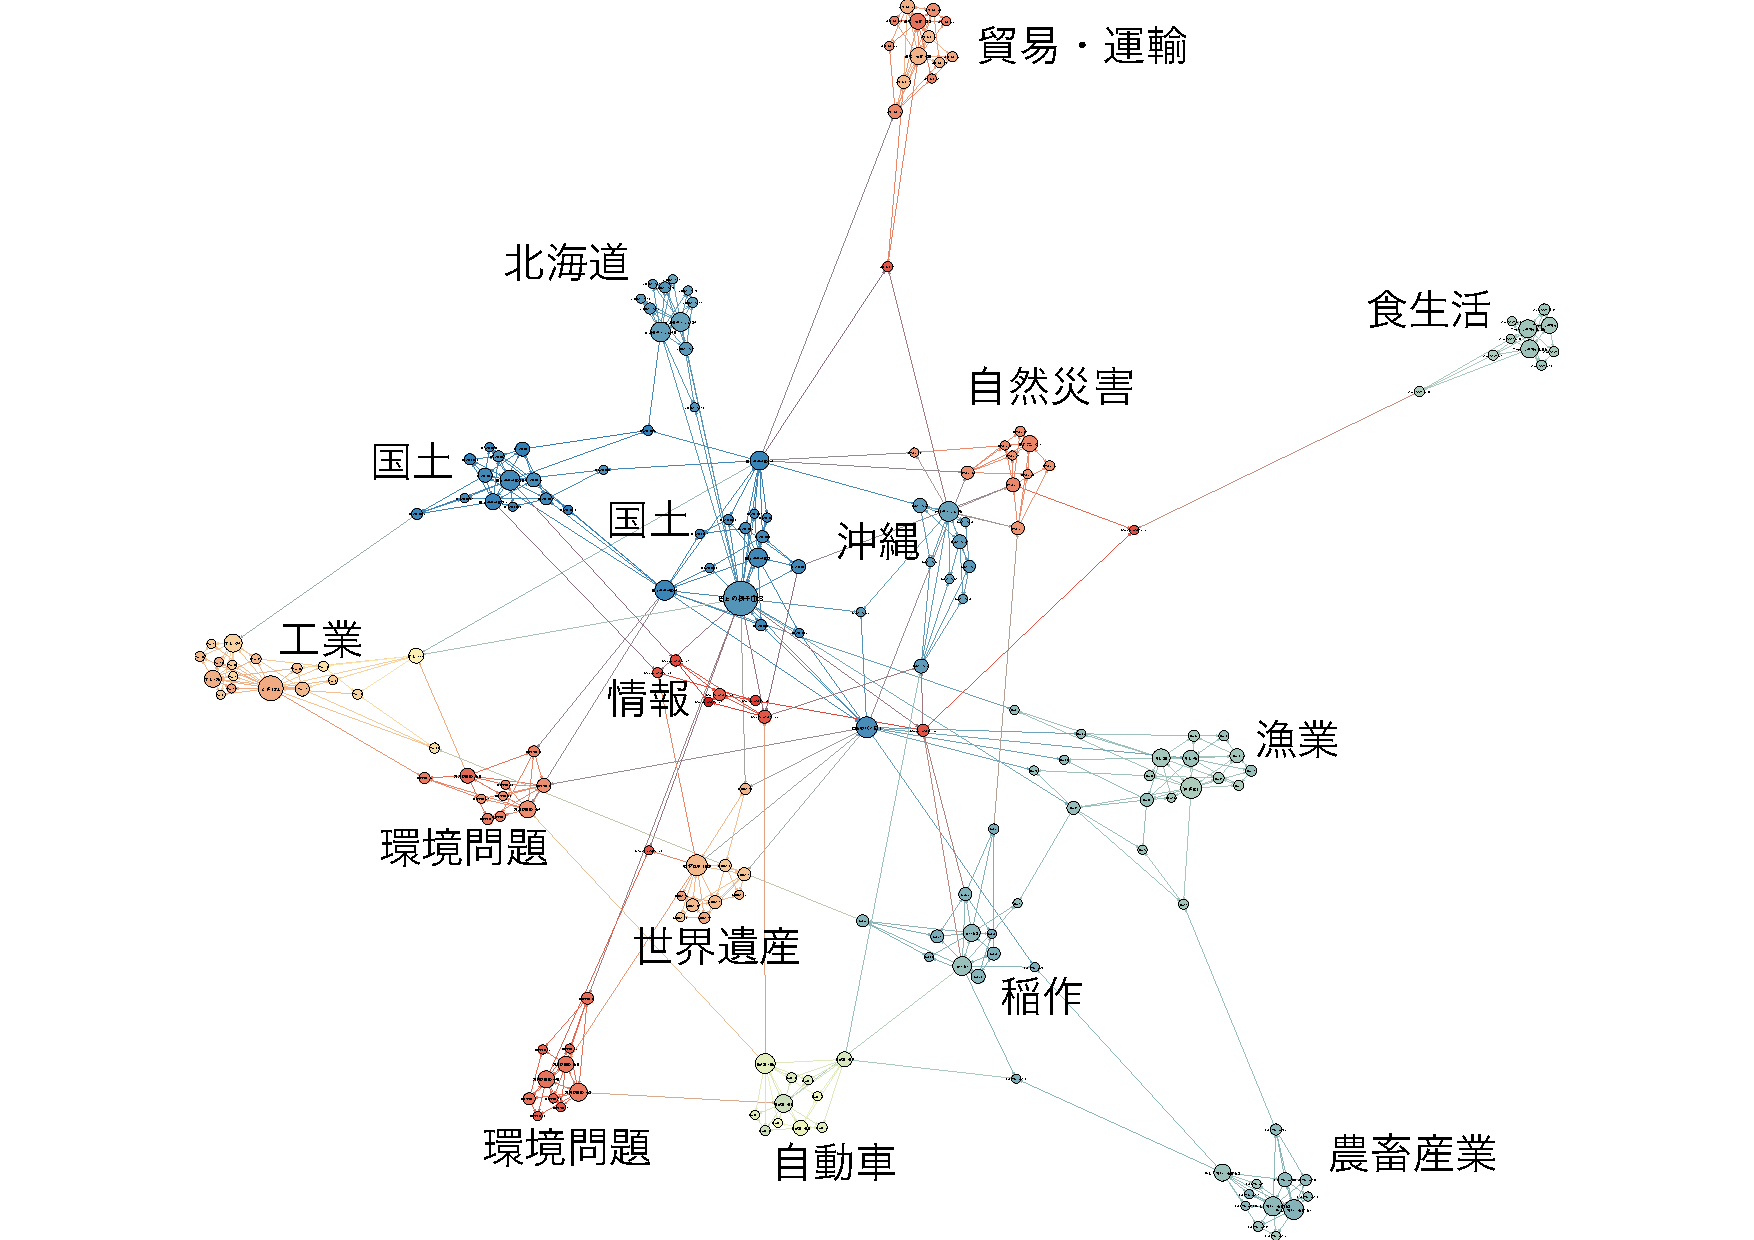
\includegraphics[width=210pt]{./img/s5_soc_label2.pdf}
			\caption{小学5年社会の知識間関係ネットワーク}
			\label{fig:net_s5soc}
		\endminipage\hfill
		\minipage{0.50\textwidth}
			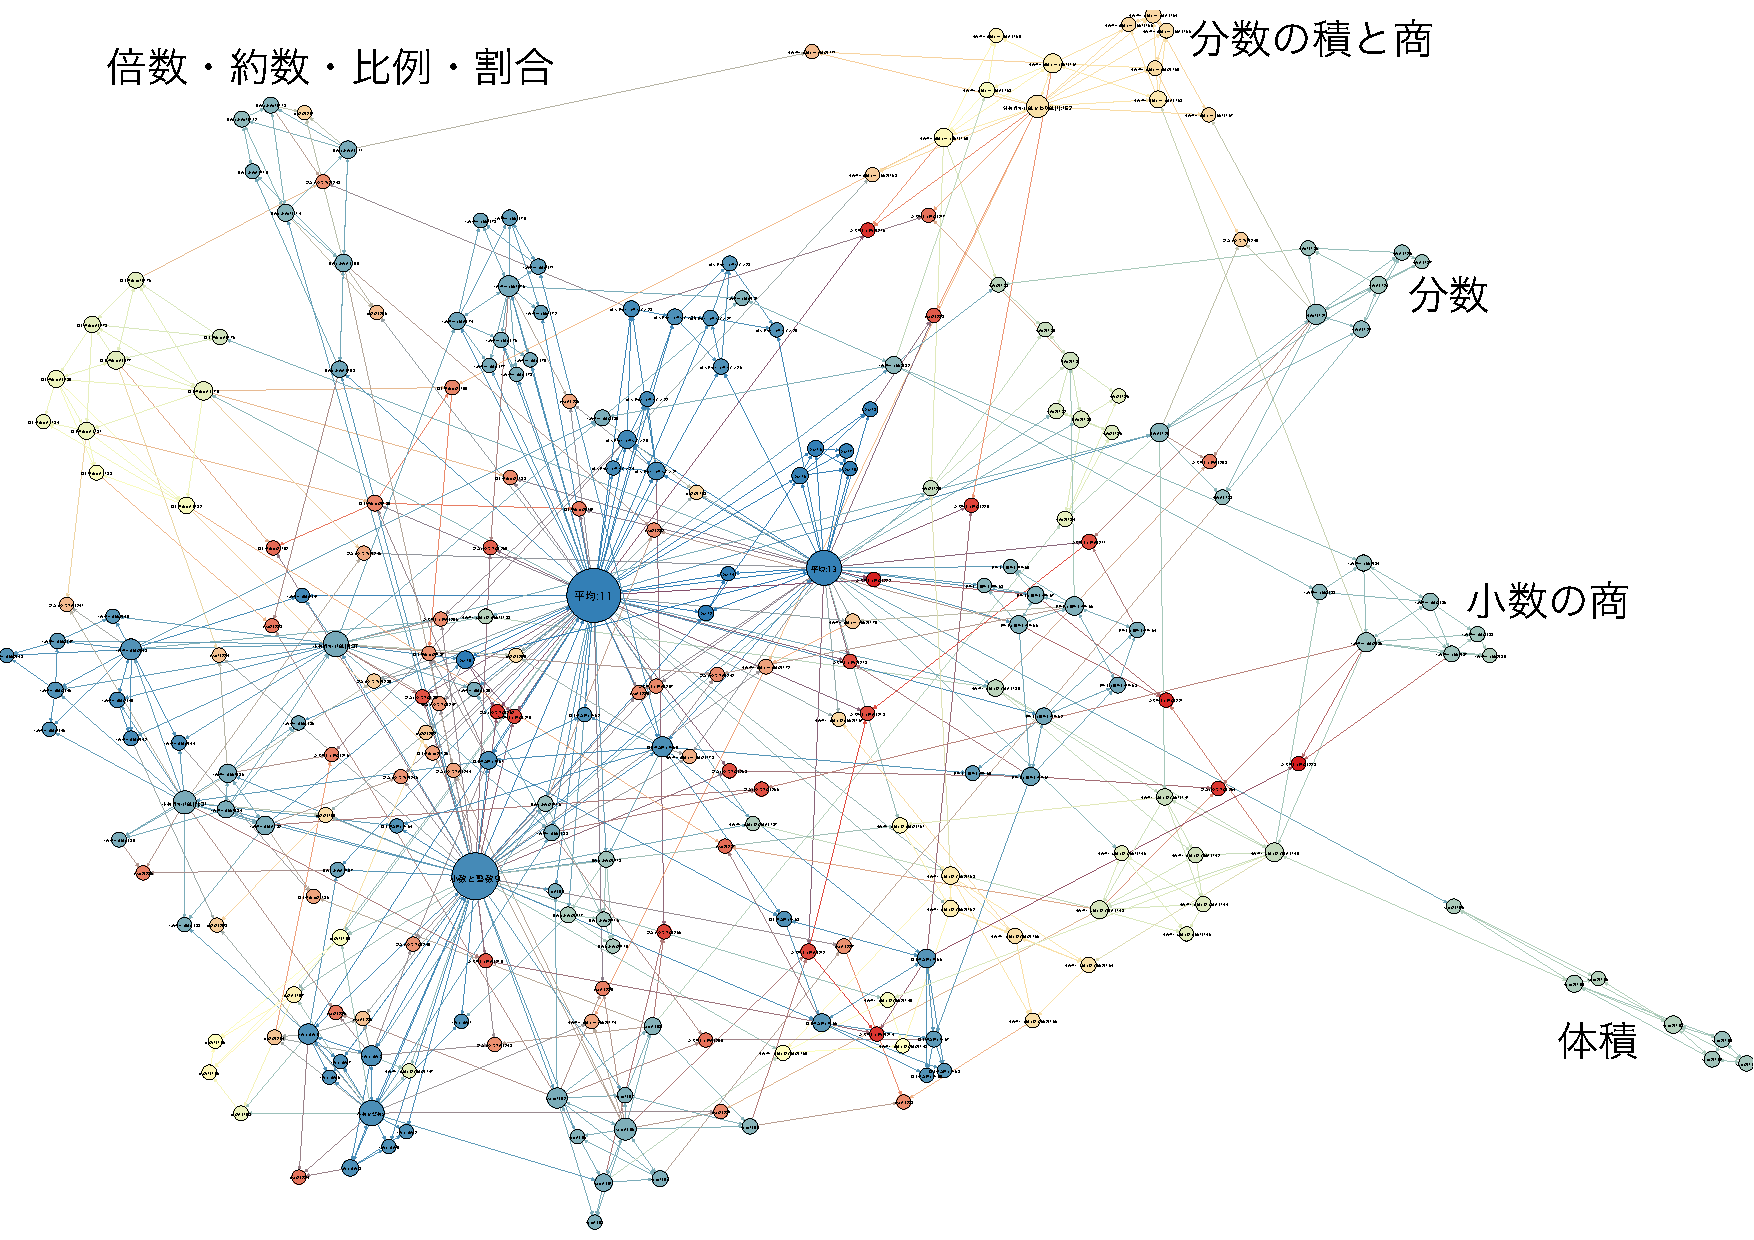
\includegraphics[width=210pt]{./img/s5_mat_label2.pdf}
			\caption{小学5年算数の知識間関係ネットワーク}
			\label{fig:net_s5mat}
		\endminipage\hfill
	}
	\hspace*{-00pt}\makebox[1.1\textwidth][c]{
		\minipage{0.50\textwidth}
			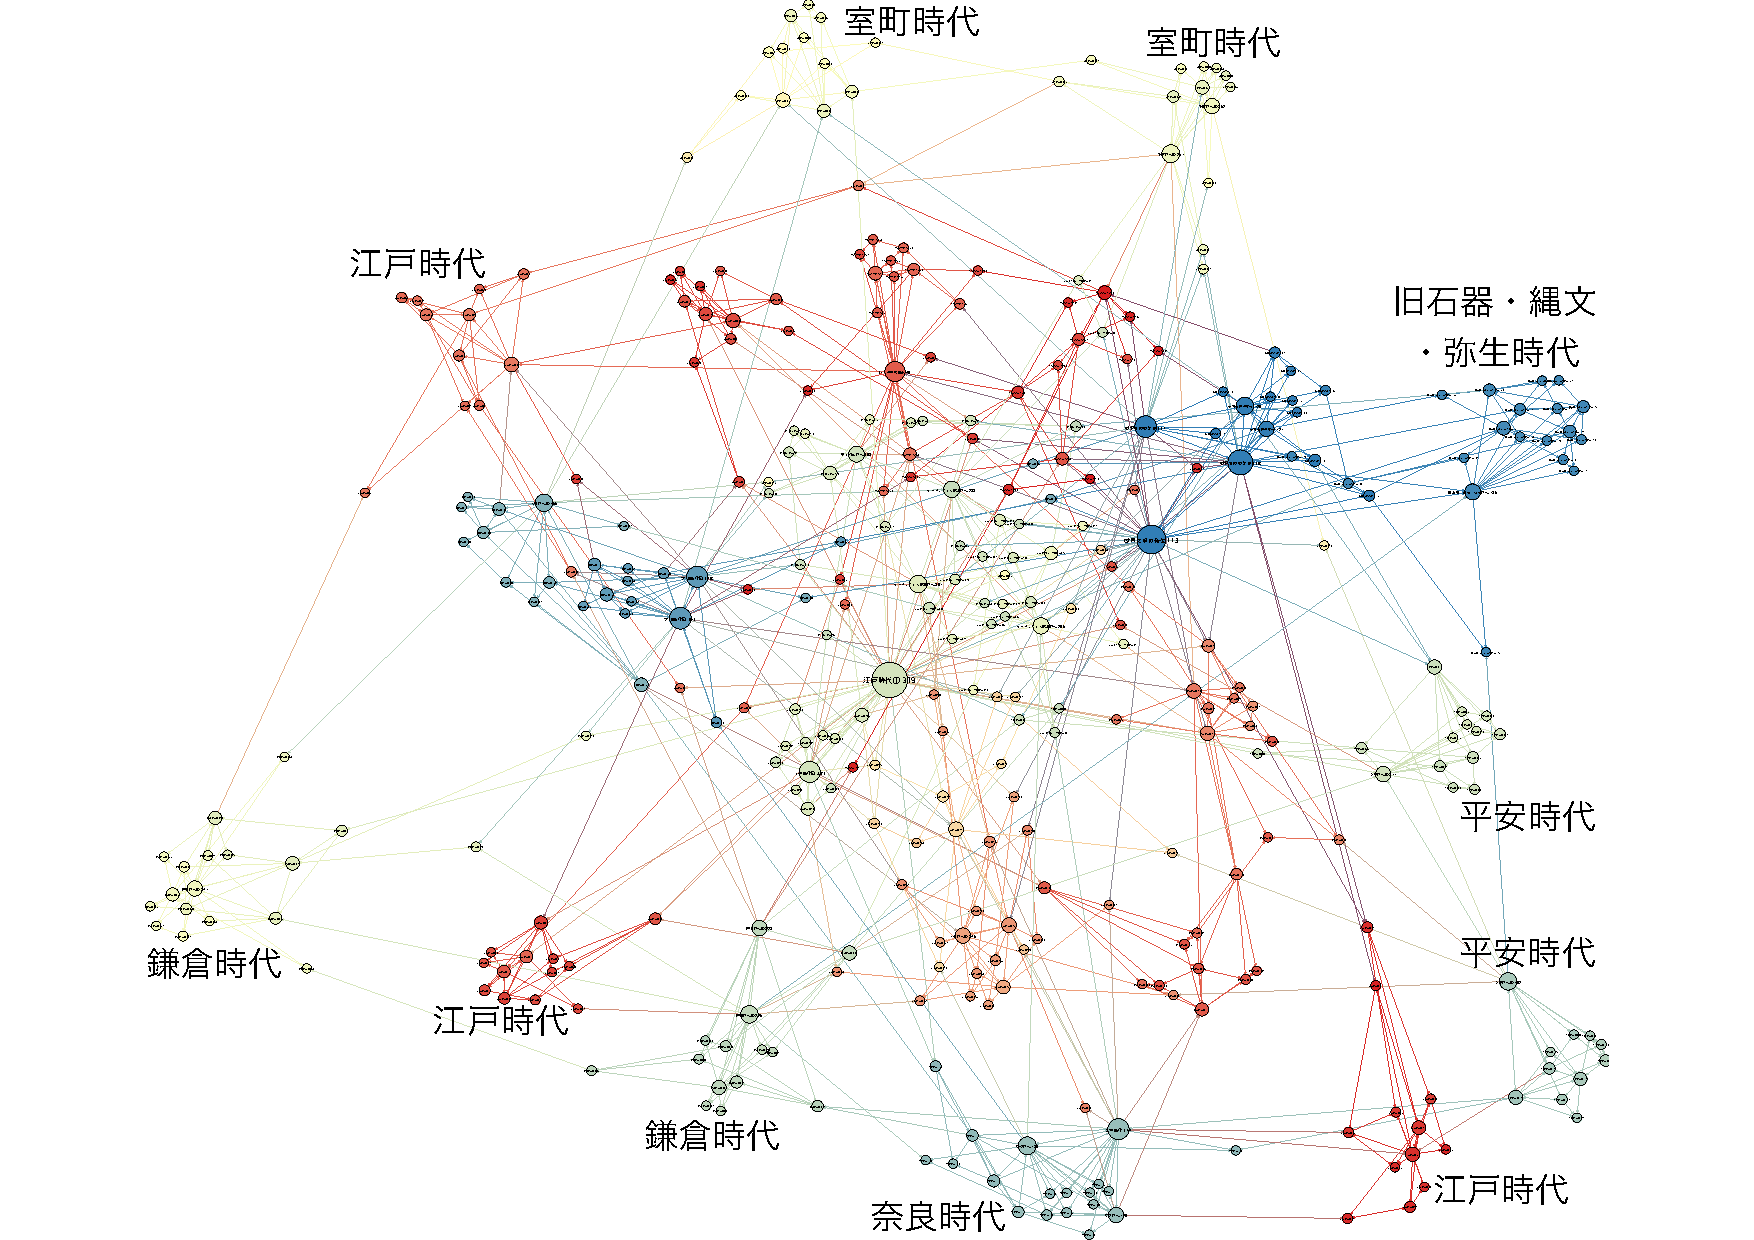
\includegraphics[width=210pt]{./img/c_his_label2.pdf}
			\caption{中学歴史の知識間関係ネットワーク}
			\label{fig:net_c_his}
		\endminipage\hfill
		\minipage{0.50\textwidth}
			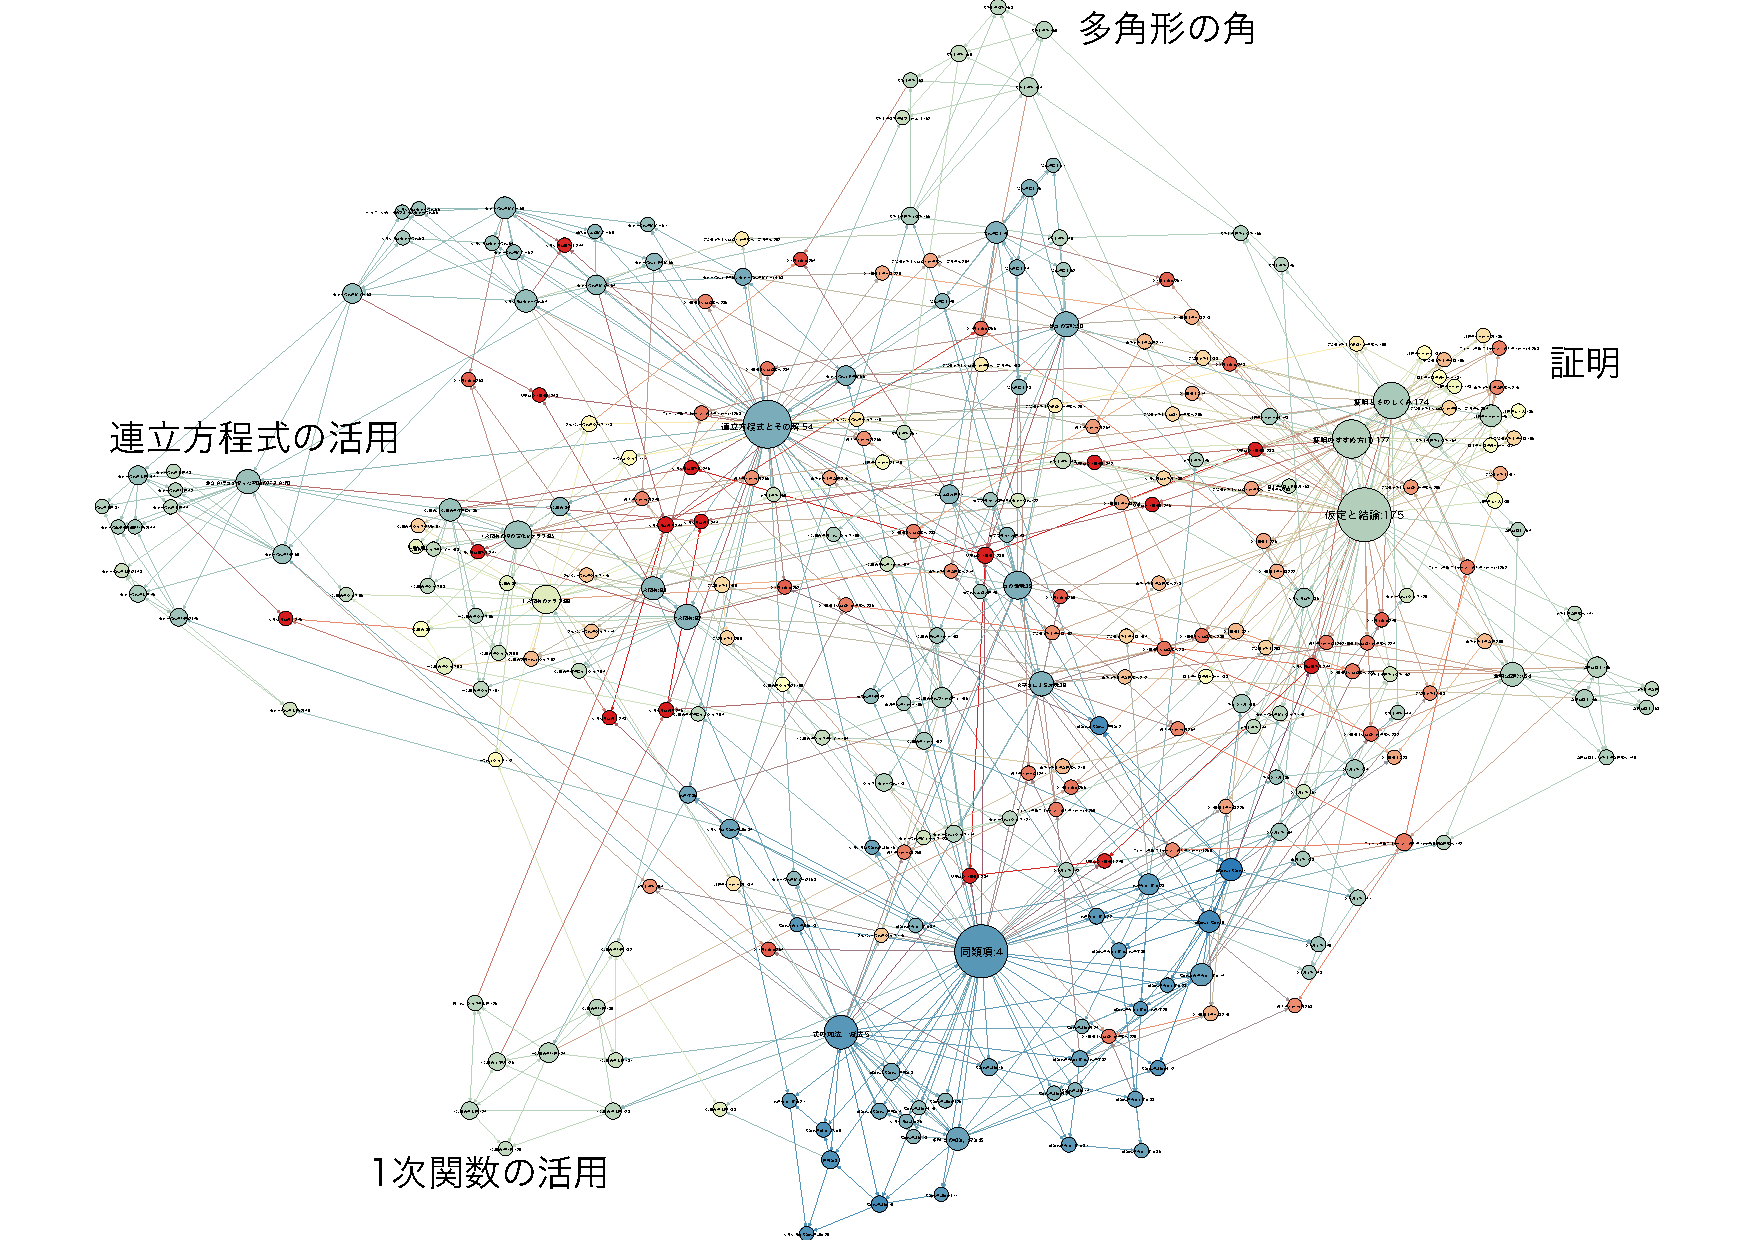
\includegraphics[width=210pt]{./img/c2_mat_label2.pdf}
			\caption{中学2年数学の知識間関係ネットワーク}
			\label{fig:net_c2mat}
		\endminipage\hfill
	}
\end{center}
\vspace*{-5mm}
\end{figure*}


小学5年社会,小学5年算数,中学歴史,中学2年数学のデータセットについて,
構築したネットワークをそれぞれ図\ref{fig:net_s5soc},\ref{fig:net_s5mat},\ref{fig:net_c_his},\ref{fig:net_c2mat}に可視化した.
ノードの内容から知識間関係を抽出できていることが分かり,
ネットワーク全体におけるノード集合の配置やその関係を内容の側面から分析し,
知識獲得における知識間関係を抽出できていることを定性的に確認した.

\begin{table}[tb]
\caption{各ネットワークにおける構造指標}
\label{tab:result2}
\begin{center}
\centerline{
{\scriptsize
\tabcolsep=0.09cm
\begin{tabular}{ccc|cc|cc|cc}\hline\hline
\multicolumn{3}{c|}{ネットワーク}	&	\multicolumn{2}{c|}{モジュラリティ}	& \multicolumn{2}{c|}{フロー階層}	&\multicolumn{2}{c}{GRC}		\\
	分類	& 科目			&				学年			&		値		&	平均			&	値		&	平均	&	値	&	平均	\\\hline
\multirow{5}{*}{\shortstack{宣言的知識\\の知識間関係\\ネットワーク}}&	\multirow{3}{*}{地理・社会}		&		小4			&	0.698	&	\multirow{5}{*}{0.759}&	0.579		&	\multirow{5}{*}{0.627}	&	0.787		& \multirow{5}{*}{0.690}\\
		&				&	小5						&	0.801	&	&	0.541	&	&	0.679		&			\\
		&				&				中学			&	0.759	&	&	0.633	&	&	0.603		&			\\\cdashline{2-3}
		&\multirow{2}{*}{歴史・社会}	&	小6		&	0.808	&	&	0.607	&	&	0.613		&			\\
		&				&				中学			&	0.728	&	&	0.774	&	&	0.768		&			\\\hdashline
%
\multirow{6}{*}{\shortstack{手続き的知識\\の知識間関係\\ネットワーク}}&		\multirow{6}{*}{算数・数学}&	小4			&	0.660	&	\multirow{6}{*}{0.602}	&	0.590	&	\multirow{6}{*}{0.756}	&	0.683	&	\multirow{6}{*}{0.816} \\
		&				&				小5			&	0.602	&	&	0.757	&	&	0.901	&			\\
		&				&				小6			&	0.688	&	&	0.705	&	&	0.875	&			\\
		&				&				中1			&	0.566	&	&	0.805	&	&	0.803	&			\\
		&				&				中2			&	0.559	&	&	0.830	&	&	0.818	&			\\
		&				&				中3			&	0.538	&	&	0.847	&	&	0.861	&			\\
%
\hline\hline
\end{tabular}
}
}
\end{center}
\end{table}

各ネットワークのモジュラリティとフロー階層,GRCを
表\ref{tab:result2}に示す.
宣言的知識の知識間関係ネットワークと手続き的知識の知識間関係ネットワークにおける
モジュラリティ,フロー階層,GRCそれぞれについて,
t検定を実施し統計的に有意な差があるかを検証した.
モジュラリティにおけるp値は$0.00106$で,
フロー階層におけるp値は$0.0482$で,
GRCにおけるp値は$0.0470$
であった.
したがって,いずれの指標においても有意水準$0.05$で有意な差が認められた.
このことは
知識獲得における知識構造について,
宣言的知識のモジュール性が手続き的知識のモジュール性より統計的に有意に高く,
逆に,
手続き的知識の階層性が宣言的知識の階層性より統計的に有意に高いことを示している.

\section{考察}
実験では,小学4年算数のデータセットから構築したネットワークは,
モジュール性が大きく階層性が小さかった.
このことは,小学4年算数が手続き的知識の獲得を主目的としていないということ意味するのではないと考える.
小学4年算数のネットワークでは複数のクラスタが存在していた.
これらのクラスタ内ではある程度の階層性が存在するが,
一方で,クラスタ間については,その内容が強く関連しているというわけではなく,
その結果,ネットワーク全体としてはモジュール性が高く,階層性が低くなってしまっているのだと推察する.



\section{結論}
本論文では,
心理学で議論されていた宣言的知識と手続き的知識の獲得における知識構造の違いを定量的に分析し,
知識獲得における宣言的知識の知識構造は手続き的知識の知識構造と比べてよりモジュール性が高く,
逆に,手続き的知識の知識構造は宣言的知識の知識構造と比べてより階層性が高いことを検証した.

本研究は
MOOCsの登場,ネットワーク分析の発展,深層学習の躍進等,
ここ数年の幅広い領域のさまざまな成果によって,初めてその実施が可能になったものである.
本研究が,人間の学習や知能の解明の一助になると信じている.









%\bibliographystyle{junsrt}
%\bibliographystyle{abbrv}
\bibliographystyle{acm}
\bibliography{biblio}




\end{document}

